\begin{figure}
\begin{center}
    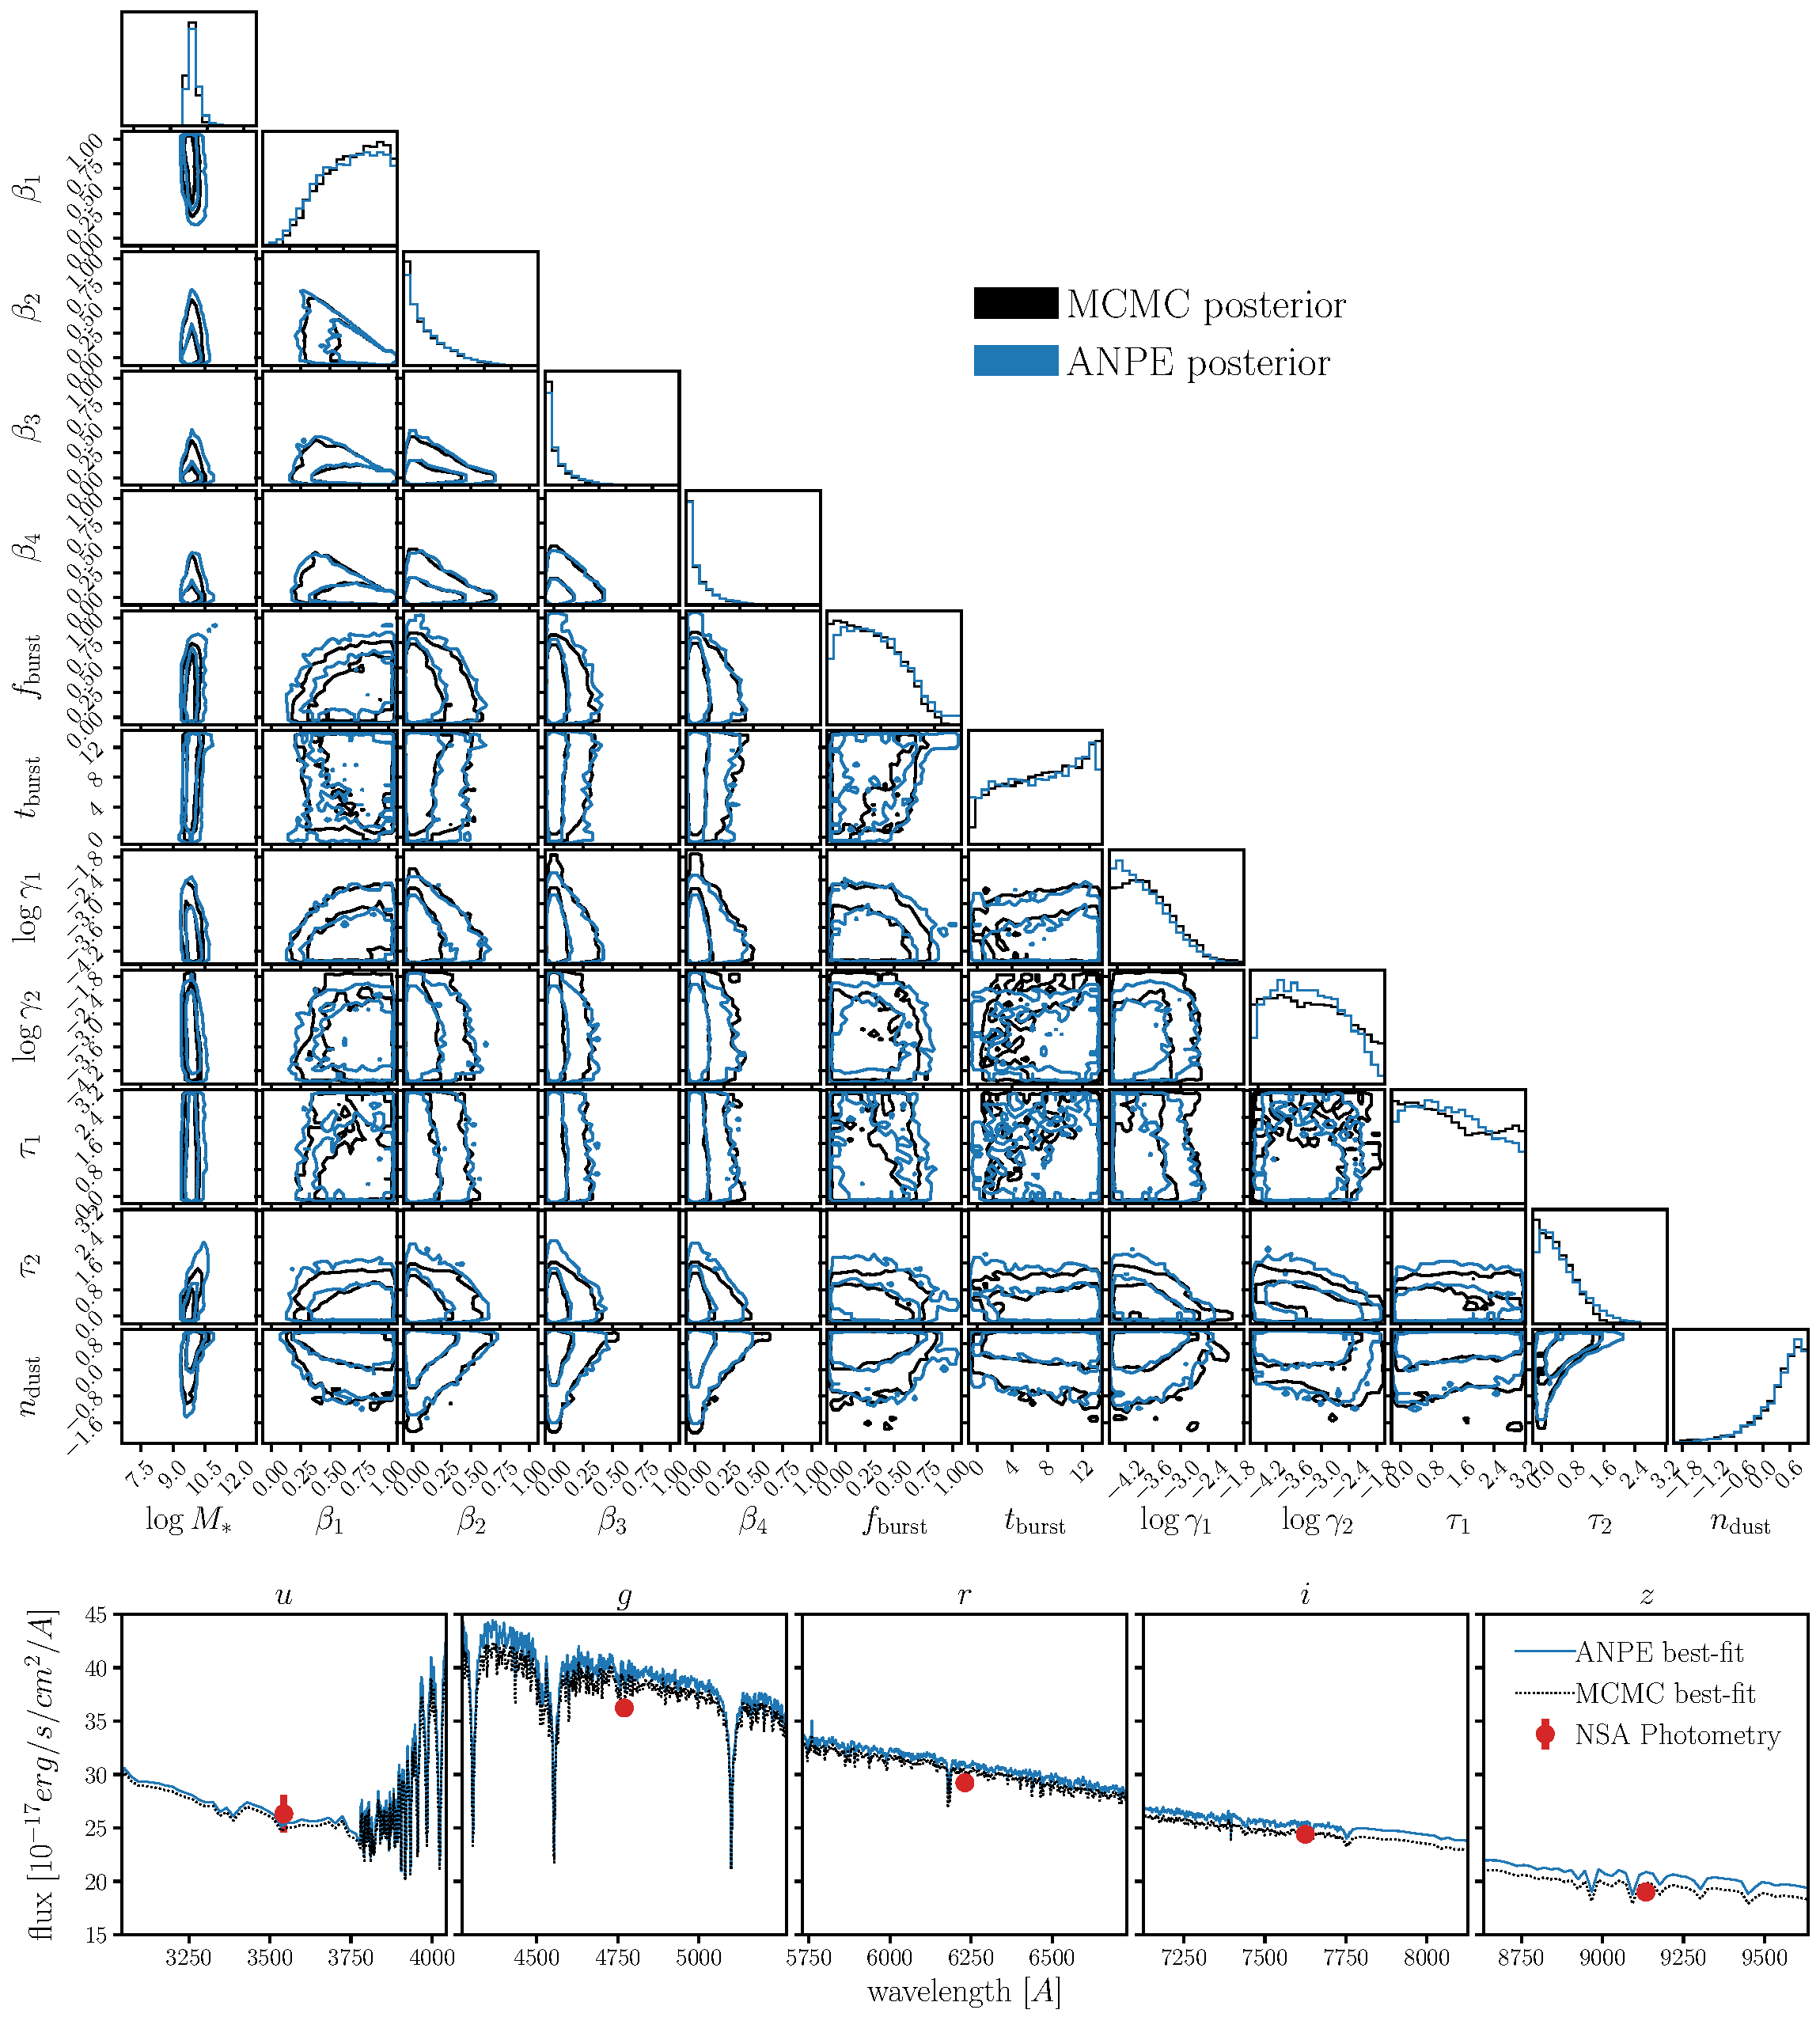
\includegraphics[width=0.9\textwidth]{figs/corner.pdf}
    \caption{\label{fig:corner}
    A comparison of the posteriors of the 12 SED model parameters derived from
    standard MCMC sampling (black) and our ANPE (blue) for a single arbitrarily
    selected NSA galaxy.
    The posteriors are in excellent agreement for all of the parameters. 
    Estimating the posterior using MCMC sampling requires X hours. 
    Even using neural emulators to accelerate likelihood evaluations, MCMC
    sampling requires Y hours. 
    \emph{With ANPE, inferring the full posterior requires 1 second per
    galaxy.}
    }
\end{center}
\end{figure}

\section{Results} \label{sec:results}
Now that we have trained our ANPE, next we validate the posteriors we infer
using it. 
We first compare the posterior from ANPE to the posterior derived from MCMC
sampling for a single arbitrarily chosen NSA galaxy in Figure~\ref{fig:corner}. 
In the top, we present the the posterior distribution of the 12 SED model
parameters (Section~\ref{sec:provabgs}) for the ANPE posterior (blue) and MCMC
posterior (black). 
The MCMC posterior is derived using the {\sc Zeus} ensemble
slice-sampler~\citep{karamanis2020} with 30 walkers and 10,000 iterations,
2,000 of which we discard for burn-in. 
The MCMC posterior takes $\sim$50 hours to derive.
Meanwhile, \emph{the ANPE posterior takes $1$ second to derive and shows
excellent agreement over the full SED parameter space}. 
 
In the bottom of Figure~\ref{fig:corner}, we compare the SED distributions of
the best-fit parameter values from the ANPE (blue) and MCMC posteriors (black
dotted). 
We also include the NSA photometric flux of the selected galaxy (red) and mark
the optical broadband response curves (dashed). 
The best-fit SED from the ANPE posterior is also in good agreement with both
the MCMC best-fit and the NSA photometry.  

% separate paragraph highlighting the computational advantage? 

\begin{figure}
\begin{center}
    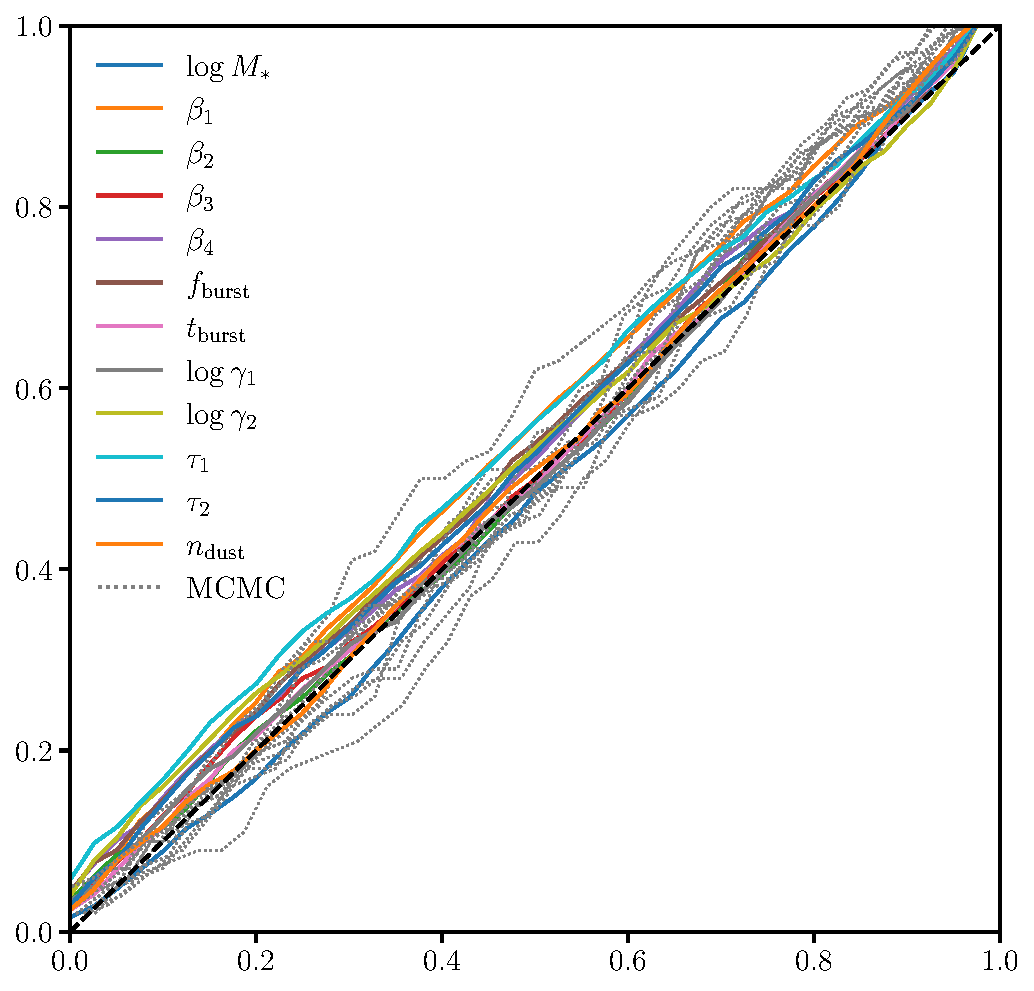
\includegraphics[width=0.5\textwidth]{figs/ppplot.pdf}
    \caption{\label{fig:pp}
    Probability-probability (p-p) plot of the ANPE for 1000 simulated test data. 
    For each SED parameter, we plot the cumulative distribution function (CDF) of the
    percentile score of the true value within the ANPE marginalized posterior.
    For the true posteriors, the percentile score is uniformly distributed so
    the CDF is diagonal (black dashed).
    The test data is constructed in the same way as the training data
    (Section~\ref{sec:training}). 
    For reference, we include the p-p plot of the posterior estimated from MCMC
    sampling (gray). 
    \emph{The ANPE is in good agreement the true posterior.}
    }
\end{center}
\end{figure}
Besides the selected NSA galaxy in Figure~\ref{fig:corner}, the posteriors from
ANPE and MCMC are overall in excellent for NSA galaxies.
However, we do not know the true SED parameters for these galaxies so to
further validate the ANPE posteriors, we use test synthetic photometry where
we know the truth.
We construct 1000 synthetic NSA galaxy photometry in the same way as the
training data in Section~\ref{sec:training} and then generate posteriors for
each of them using our ANPE. 

In Figure~\ref{fig:pp}, we present the probability-probability (p-p) plot of
the ANPE posteriors for the test data. 
The p-p plot presents the cumulative distribution function (CDF) of the
percentile score of the true value within the marginalized posterior for each
SED parameter. 
For the true posterior, the percentiles are uniformly distributed so the CDF
is a diagonal, which we include in black dashed.
\emph{Overall, the ANPE posteriors are in good agreement with the true
posteriors for each of the SED parameters}.

We also include in Figure~\ref{fig:pp} the CDFs of the SED parameters for the
MCMC posteriors derived for a subset of 100 test galaxy photometry (gray
dotted). 
Based on the CDFs, the ANPE posteriors are in actually better agreement with
the true posteriors than those derived from MCMC.
This is due to the fact that MCMC posteriors are only estimates of the true
posterior and are subject to limitations in initialization, sampling, and
convergence.
Meanwhile, these limitations do not impact posteriors from ANPE and so the
comparison highlights additional advantages of ANPE besides the $10^5\times$
speed up.

\begin{figure}
\begin{center}
    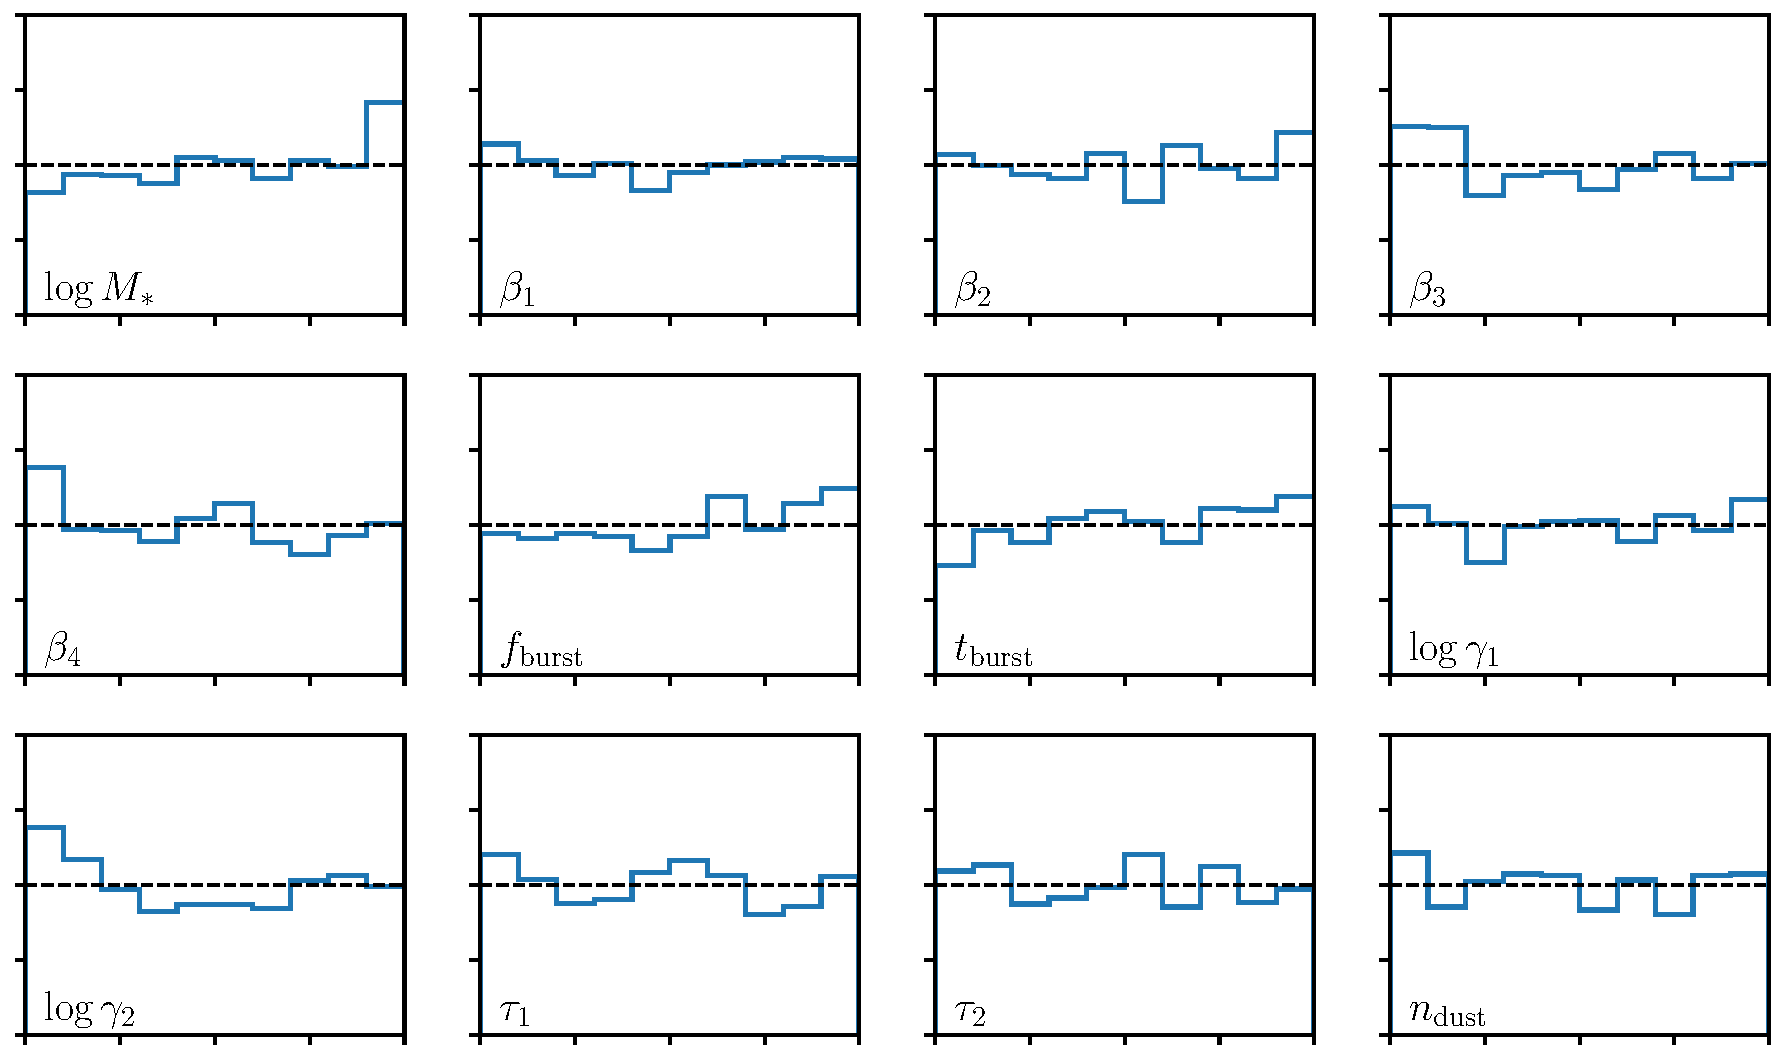
\includegraphics[width=0.9\textwidth]{figs/sbc.pdf}
    \caption{\label{fig:sbc}
    Simulation-based calibration plot of the ANPE for 1000 simulated test data. 
    For each SPS parameter, we plot the cumulative distribution function (CDF) of the
    percentile score of the true value within the ANPE marginalized posterior.
    For the true posteriors, the percentile score is uniformly distributed so
    the CDF is diagonal (black dashed).
    The test data is constructed in the same way as the training data
    (Section~\ref{sec:training}). 
    For reference, we include the p-p plot of the posterior estimated from MCMC
    sampling (gray). 
    \emph{The ANPE is in good agreement the true posterior.}
    }
\end{center}
\end{figure}

In Figure~\ref{fig:sbc}, we present another validation of the ANPE posteriors
using simulation-based calibration~\citep[SBC;][]{talts2020}. 
% what are the advantages of SBC? --- i.e. why do we show this in addition to
% pp plot? 
% SBC a general procedure for validating inferences from Bayesian algorithms capable of generating posterior samples. This procedure not only identifies inaccurate computation and inconsistencies in model implementations but also provides graphical summaries that can indicate the nature of the problems that arise. 

